\section{Dominators}
\frame{

\frametitle{\secname}
\begin{columns}
\column{0.6\textwidth}
\begin{itemize}
\item<1-> Analysis of control-flow graphs
\item<1-> Node $A$ dominates $B$ if any path from the entry node to $B$ must pass through $A$.
\item<1-> Any node dominates itself; to exclude this case, use strict dominance.
\item<1-> Strict dominance cannot have a cycle
\begin{itemize}
\item<1-> Suppose $A$ dominates $B$
\item<1-> Take a path to $B$ with no cycles
\item<1-> Shorten this path so it ends at $A$
\item<1-> This is a path from the entry node to $A$ that doesn't pass through $B$.
\end{itemize}
\item<2-> The strict dominance graph can be top-sorted
\end{itemize}

\column{0.4\textwidth}
\centering
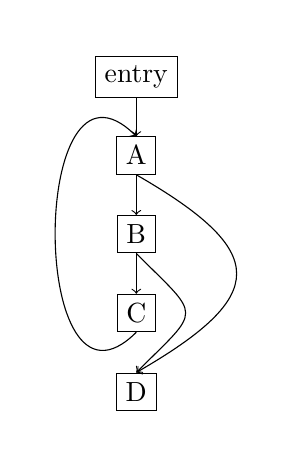
\begin{tikzpicture}
\node[draw] (entry) {entry};
\node[draw,below of=entry] (A) {A};
\draw[->] (entry) -- (A);
\node[draw,below of=A] (B) {B};
\draw[->] (A) -- (B);
\node[draw,below of=B] (C) {C};
\draw[->] (B) -- (C);
\draw[->,tips=on proper draw] (C.south) edge [out=225,in=135,looseness=2] (A.north);
\node[draw,below of=C] (D) {D};
\draw[->,tips=on proper draw] (A.south) edge [out=-30,in=30,looseness=2] (D.north);
\draw[->,tips=on proper draw] (B.south) edge [out=-45,in=45,looseness=2] (D.north);

\end{tikzpicture}

\end{columns}

}
